\chapter{Instructions for Installation}

After you have started Eclipse 3.0, change to CVS Repositories perspective and add a CVS repository. \par
Enter the following data (see \ref{neuesrep}):
\begin{itemize}
\item host: cvs.berlios.de
\item repository path: /cvsroot/kobold
\item user: anonymous
\end{itemize}
Leave the remaining data untouched and confirm the dialog. \par

\begin{figure}[h!]
\begin{center}
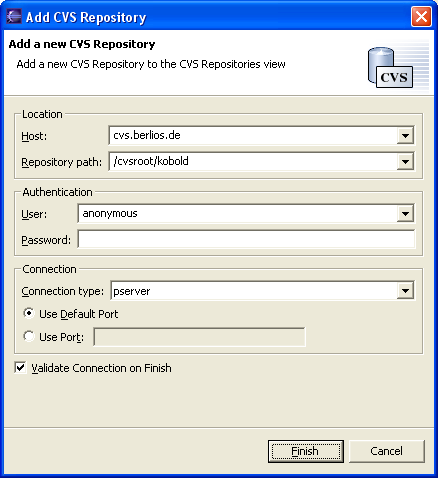
\includegraphics[width=12cm]{neuesrep.png}
   \caption{Adding a new repository}�
\label{neuesrep}
\end{center}
\end{figure}

Open the tree along HEAD, kobold and src (see \ref{auschecken}). Check out the four folders kobold.client.plam,
kobold.client.vcm, kobold.common and kobold.server through 'check out as..' (context menue)
and confirm with 'Finish'.

\begin{figure}[h!]
\begin{center}

\includegraphics[width=10cm]{auschecken.png}
   \caption{This is how your tree should look like}
\label{auschecken}
\end{center}
\end{figure}\par

Open the 'Window' menu and select 'preferences'. Select 'plug-in development' and 'Target 
Platform' and press the button 'Not in Workspace'. Confirm with OK. \par

Projects kobold.client.plam, kobold.client.vcm and kobold.common: \par
Right-click on the project and select 'properties'. Select 'Java build path' and the 'source'
tab. Remove the existing entry and add a new one by pressing 'Add Folder'. Choose the 
src-folder and confirm. Append '/bin' to the default output folder (see \ref{buildpath}).
 Close the preferences dialog. \par

\begin{figure}[h!]
\begin{center}
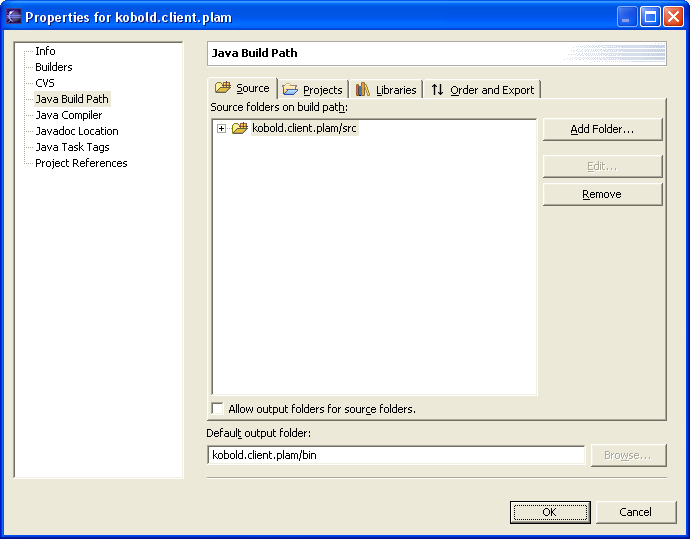
\includegraphics[width=15cm]{buildpath.png}
   \caption{This is how your buildpath should look like}
\label{buildpath}
\end{center}
\end{figure}\par

Projects kobold.server: \par
Right-click on the project and select 'properties'. Select 'Java build path' and the 'source'
tab. Remove the existing entry and add a new one by pressing 'Add Folder'. Choose the 
src-folder and confirm. Append '/bin' to the default output folder. 
Switch to the 'projects' tab and select 'kobold.common'. Close the preferences 
dialog. \par

Again, right-click on the project kobold.client.plam and select 'update classpath'. Select 
kobold.client.plam, kobold.client.vcm and kobold.common and confirm.
